\documentclass[main.tex]{subfiles}

\begin{document}

\listoftodos

\section*{Appendix: Bellman and CEC parameter comparisons}\label{sec:parameter_comparison}
This article contains many numerical experiments on a system
with a fixed combination of the five parameters:
Termination time $T$, unsold items cost $C$, uncertainty $\gamma$, and
demand function parameters $q_1,q_2$.
In this section we explore the differences between the Bellman policy
and the CEC policy for a larger parameter range.
We are interested in the difference between the profit following
a Bellman policy $\alpha^B$ and a CEC policy $\alpha^C$.
The policy $\alpha^B$ is computed numerically, and
$\alpha^C$ is obtained using the function $a^C$ from
the formula in \Cref{eq:cec_policy}.
As a reminder, the profit of following a policy process $\alpha$ is
the random variable
\begin{equation}
  P^\alpha = \sum_{t=0}^{T-1}\alpha_tQ(S_t^\alpha,\alpha_t,W_{t+1}) - CS_T^\alpha.
\end{equation}
In particular, the difference between the two policies is measured
using the $L^2$-norm with respect to the probability distribution
induced by the disturbance $(W_1,W_2,\dots,W_T)$, that is
\begin{equation}
  \left\|P^{\alpha^B}-P^{\alpha^C}\right\|_2
  =\sqrt{\mathbb E_W\left[{( P^{\alpha^B}-P^{\alpha^C} )}^2 \right]}.
\end{equation}

To reduce the number of combinations of parameters, we make the
simplification to choose only
four combinations of
$(C,\gamma)\in\{0.5,1\}\times\{0.05,0.1\}$.
Then,
for each combination of $(C,\gamma)$,
we can create a heatmap of the difference between the two policy
functions by varying the parameters $q_1,q_2$.
The relative $L^2$ difference between the CEC and Bellman policy outcomes
is shown in \Cref{fig:profit_diff_heatmaps}. The norms were approximated
with $1000$ samples from $(W_1,W_2,\dots,W_T)$.
Comparing the left and right column, we see that the relative difference doubles as
the standard deviation $\gamma$ is doubled. The cost $C$ plays a large
role, both in terms of the shape of the difference surface and its
magnitude.
The black region at the bottom right of the plots correspond to popular,
low-elasticity products where both policies choose to sell at the
maximum price $a=1$.
\begin{figure}[htbp]
  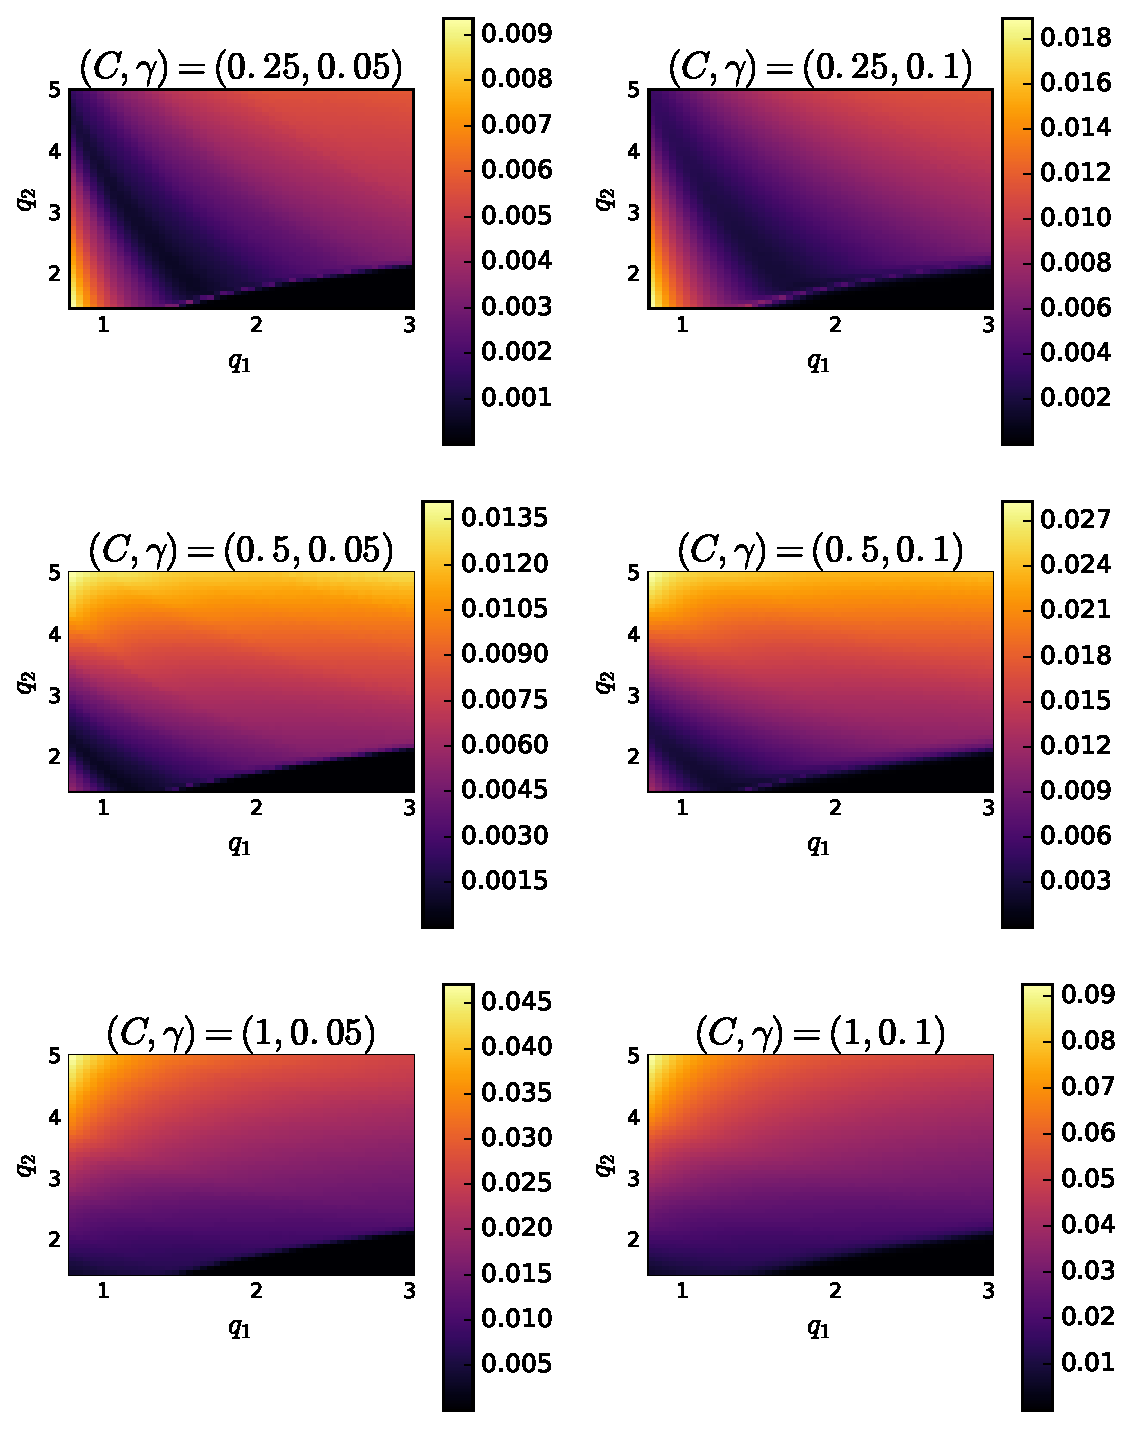
\includegraphics[width=\textwidth]{./img/profit_diff_heatmaps}
  \caption{The relative $L^2$ difference
    $\|P^{\alpha^B}-P^{\alpha^C}\|_2/\|P^{\alpha^B}\|_2$ representing
    how different the CEC policy is to the optimal Bellman policy.
    Each plot defines a combination of $(C,\gamma)$, whilst
    the axes vary the parameters $q_1,q_2$ of the demand function
    $q(a)=q_1e^{-q_2a}$.
    The white dot on the bottom, left plot corresponds to the
    parameters chosen for the experiments in this article.
  }\label{fig:profit_diff_heatmaps}
\end{figure}

The parameters chosen in this article's numerical experiments
are $C=1,\gamma=0.05,q_1=e^2/3\approx2.5,q_2=3$. This point lies
in the region where the relative difference is around $0.016$ --- see the
white dot in the
bottom, left subfigure in \Cref{fig:profit_diff_heatmaps}.
This difference is in the middle of that seen for all the
combinations of parameters, so the conclusions made in the article
should be considered as relevant for a wider range of systems.
\Cref{tbl:paramcomparisons} provides further data to underscore
the claim that the CEC policy
outperforms the Bellman policy the
majority of events, at the expense of a stronger underperformance
for the remainder of the events. Notably, the CEC policy is better
more than 50\% of the time for all the parameter
combinations considered in this article. The values in
\Cref{tbl:paramcomparisons} were approximated using $10,000$ samples
from $W$, and their corresponding parameter combinations are shown as
grey dots in \Cref{fig:profit_diff_heatmaps}.

\begin{table}[htbp]
  \centering
  \begin{tabular}{llllcccc}
    $C$ & $\gamma$ & $q_1$ & $q_2$ & $\mbox{VaR}_{0.05}$
    &Median & $\mbox{VaR}_{0.95}$ &$L_2$\\
    \toprule
    $0.25$ & $0.05$ & $2.0$ & $4.0$ & -0.4 & -0.3 & 0.6 & 0.4 \\
    $0.25$ & $0.1$ & $1.33$ & $2.67$ & -0.5 & -0.0 & 0.6 & 0.3 \\
    $0.5$ & $0.05$ & $2.67$ & $4.0$ & -0.6 & -0.6 & 1.9 & 1.1 \\
    $0.5$ & $0.1$ & $2.0$ & $2.67$ & -0.9 & -0.6 & 1.9 & 1.2 \\
    $1.0$ & $0.05$ & $1.33$ & $4.0$ & -1.2 & -1.1 & 5.3 & 2.7 \\
    $1.0$ & $0.1$ & $2.67$ & $2.67$ & -1.5 & -1.3 & 5.8 & 2.9\\
    &&&&$\times 10^{-2}$&$\times 10^{-2}$&$\times 10^{-2}$&$\times 10^{-2}$\\
    \bottomrule
  \end{tabular}
  \caption{Statistics comparing $P^{\alpha^B}$ and $P^{\alpha^C}$ for six different
    parameter combinations. The columns $\mbox{VaR}_s$ represent the
    $s$-Value-at-Risk, or the $s^{\text{th}}$ quantile of the relative
    difference
    $1-P^{\alpha^C}/P^{\alpha^B}$. Median is the same as $\mbox{VaR}_{0.5}$.
    The values in the column $L_2$ refers to the relative $L_2$
    difference $\|P^{\alpha^B}-P^{\alpha^C}\|_2/\|P^{\alpha^B}\|_2$
    from \Cref{fig:profit_diff_heatmaps}. Each of the parameter
    combinations correspond to a gray dot in \Cref{fig:profit_diff_heatmaps}.
  }\label{tbl:paramcomparisons}
\end{table}
\biblio
\end{document}

%%% Local Variables:
%%% mode: latex
%%% TeX-master: t
%%% TeX-command-extra-options: "-shell-escape"
%%% End:
